\subsection{Transakce}
\begin{itemize}
\item \textbf{Logická (nedělitelná, atomická) jednotka práce s databází}, která začíná operací \textbf{BEGIN TRANSACTION} a končí provedením operací \textbf{COMMIT} nebo \textbf{ROLLBACK}.
\item Obecně zahrnuje posloupnost operací.
\item Úkolem převést \textbf{korektní stav databáze} na jiný korektní stav.
\item O řízení se stará \textbf{manager transakcí} nebo \textbf{monitor transakčního zpracování}.
\item \textbf{Commit:}
\begin{itemize}
\item Transakce doběhla úspěšně a změny mohou být \textbf{trvale uloženy}, zámky a adresace uvolněny (kromě WITH HOLD).
\item Zavádí \textbf{potvrzovací bod}.
\item Odpovídá úspěšnému ukončení logické jednotky práce a \textbf{označuje korektní stav DB}.
\end{itemize}
\item \textbf{Rollback:}
\begin{itemize}
\item Označuje, že databáze může být v \textbf{nekorektním stavu} a všechny změny transakce musí být \textbf{zrušeny}.
\end{itemize}
\item Operace transakce jsou nejprve zaznamenávány do\textbf{ logu}.
\item Transakce nemohou být vnořovány.
\item \textbf{Záchranné body:}
\begin{itemize}
\item Umožní \textbf{rollback} do zácharného bodu v rámci transakce. Nedochází ke zrušení celé transakce.
\item Existuje pouze v kontextu transakce.
\end{itemize}
\end{itemize}

\subsection{Zotavení}
\begin{itemize}
\item Nastává po \textbf{chybě SŘBD} => Zotavení databáze z nějaké chyby.
\item Výsledkem musí být \textbf{korektní stav DB}.
\item Využívají se\textbf{ skryté redundantní} informace.
\item Jednotkou zotavení je \textbf{transakce}.
\item Všechny změny jsou zapisovány do logu \textbf{před zápisem změn do DB} => \textbf{pravidlo dopředného zápisu do logu}.
\item Do logu se zapisuje \textbf{sekvenčně}, proto poskytuje \textbf{vyšší výkon} než přímý zápis dat.
\end{itemize}

\subsubsection{Chyby zotavení}
\begin{itemize}
\item\textbf{Lokální} - pouze v rámci jedné transakce (chyba v dotazu, přetečení hodnoty atributu).
\item\textbf{Globální} - ovlivňují více transakcí najednou:
\begin{itemize}
\item\textbf{Systémové (soft crash)} (výpadek proudu, pád systému).
\item\textbf{Chyby média (hard crash)} - chyba disku (zotavení probíhá ze záložní kopie a z logu jsou obnoveny potvrzené transakce po vytvoření zálohy).
\end{itemize}
\end{itemize}

\subsubsection{Průběh zotavení}
Základním problémem vzniklým při systémové chybě je ztráta obsahu hlavní paměti, tedy ztráta obsahu vyrovnávací paměti SŘBD. Přesný stav transakce přerušené chybou není znám a transakce musí být \textbf{zrušena} (\textbf{UNDO}). Někdy je transakce úspěšně dokončena, ovšem změny, nejsou přeneseny z vyrovnávací paměti na disk. V tomto případě musí být transakce po restartu systému přepracována (\textbf{REDO}). \textbf{Typy zotavení}: 

\begin{itemize}
\item Zotavení \textbf{Odloženou aktualizací (deferred update, NO-UNDO/REDO)}
\begin{itemize}
\item Neprovádí aktualizace databáze na disk dokud transakce nedosáhne\textbf{ potvrzovacího bodu}. Všechny změny jsou v paměťovém bufferu.
\item Jakmile transakce dosáhne potvrzovacího bodu se \textbf{nejprve zapíše vše do logu} a pak do DB (\textbf{pravidlo dopředného zápisu do logu}).
\item Při selhání transakce není nutné provádět \textbf{undo}, změny jsou ztraceny spolu s vyrovnávací pamětí.
\item \textbf{Redo} se provádí při chybě během zápisu do DB.
\item Do logu jsou v případě odložené aktualizace zapsány nové hodnoty (kvůli REDO).
\item Minimální I/O operace, používá se pouze pro \textbf{krátké} a \textbf{nenáročné transakce} - \textbf{hrozí přetečení bufferu}.
\end{itemize}
\item\textbf{Okamžitou aktualizací (immediate update, UNDO/NO-REDO)}
\begin{itemize}
\item \textbf{Může provádět aktualizace DB} než transakce dosáhne potvrzovacího bodu.
\item Operace jsou zapsány do logu a poté je aktualizována DB (pravidlo dopředného zápisu do logu).
\item Při chybě je nutné provést \textbf{undo}, protože \textbf{došlo k aktualizaci DB}.
\item Do logu se zapisují \textbf{původní hodnoty}, což umožní systému provést UNDO.
\item \textbf{Velká zátěž disku}.
\end{itemize}
\item\textbf{Kombinovanou aktualizací (UNDO/REDO)}
\begin{itemize}
\item Používaná v praxi. Využívá obou operací v kombinaci s technikou kontrolních bodů.
\item Nezapisuje všechny potvrzené operace na disk, místo toho vytváří \textbf{kontrolní body}.
\begin{itemize}
\item Zápis operací hromadně po určitém počtu záznamů.
\item Zapisuje se obsah vyrovnávací paměti na disk a záznam o kontrolním bodu do logu.
\end{itemize}
\item Po restartu systému se provádí: \textbf{undo} na všechny transakce, které se \textbf{nestihly potvrdit} a \textbf{redo} na všechny transakce, které \textbf{se potvrdily} po vytvoření kontrolního bodu.
\end{itemize}
\end{itemize}

\subsection{ACID}
Každá transakce by měla splňovat následující vlastnosti:
\begin{itemize}
\item\textbf{Atomičnost (Atomicity)} – transakce musí být atomická: jsou provedeny všechny operace transakce nebo žádná.
\item\textbf{Korektnost (Correctness)} – transakce převádí korektní stav databáze do jiného korektního stavu databáze, mezi začátkem a koncem transakce nemusí být databáze v korektním stavu.
\item\textbf{Izolovanost (Isolation)} – transakce jsou navzájem izolovány: změny provedené jednou transakcí jsou pro ostatní transakce viditelné až po provedení COMMIT. 
\item\textbf{Trvalost (Durability)} – jakmile je transakce potvrzena, změny v databázi se stávají trvalými i po případném pádu systému.
\end{itemize}

\subsection{Problémy souběhu}
\begin{itemize}
\item Jednouživatelský/víceuživatelský DB systém (kolik současně)
\item Souběh umožňuje SŘBD \textbf{zpřístupnit databázi mnoha transakcím ve stejném čase}.
\item Souběh také přináší mnoho \textbf{problémů} (nutné řešit i na \textbf{aplikační}) úrovni.
\end{itemize}

\subsubsection{Plán provádění transakce a anomálie}
Plán provádění transakce = posloupnost operací transakce, při souběžném provedení - \textbf{plán souběžný/paralelní}. Vznikají \textbf{3 problémy:}
\begin{itemize}
\item \textbf{Problém ztráty aktualizace} - jedna transakce \textbf{přepíše právě prováděnou hodnotu}. Časová posloupnost: \texttt{read\_A}, \texttt{read\_B}, \texttt{write\_A}, \texttt{write\_B}.
\\\\
\noindent\makebox[\textwidth]{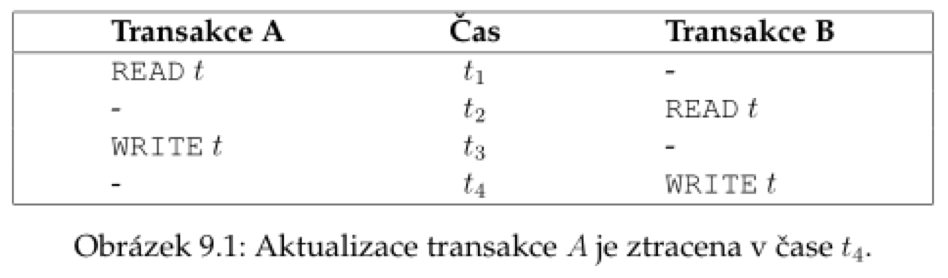
\includegraphics[width=10cm]{assets/soubeha3}}
\item \textbf{Problém nepotvrzené závislosti} - \textbf{A přečte nepotvrzená} (non-commited) data zapsaná B, B pak provede \textbf{callback}. A má \textbf{neplatná data}! Nebo B zapíše, A zapíše, B rollback - vrátí do stavu před 1. zápisem B.
\\
\noindent\makebox[\textwidth]{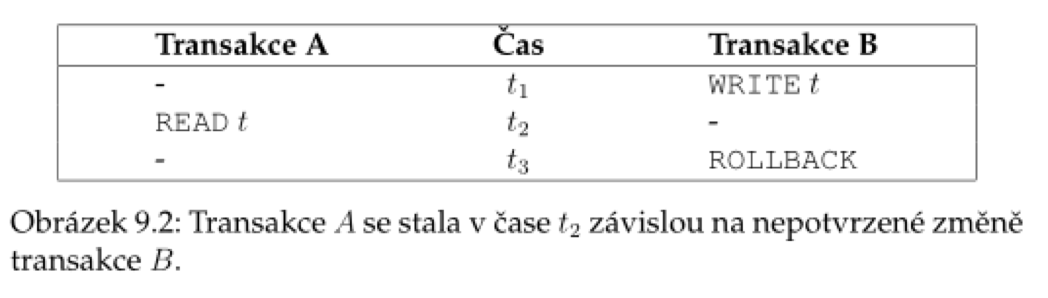
\includegraphics[width=10cm]{assets/soubeha2}}
\item \textbf{Problém nekonzistentní analýzy} - A provádí součet na účtech, před dokončením B provede přesun z účtu na účet, přičemž 1 už byl započítán a druhý ne. \textbf{Špatný součet zůstatků!} A čte commited data (B provede commit, než si A vyžádá další účet), ale i tak to není správné.
\\\\
\noindent\makebox[\textwidth]{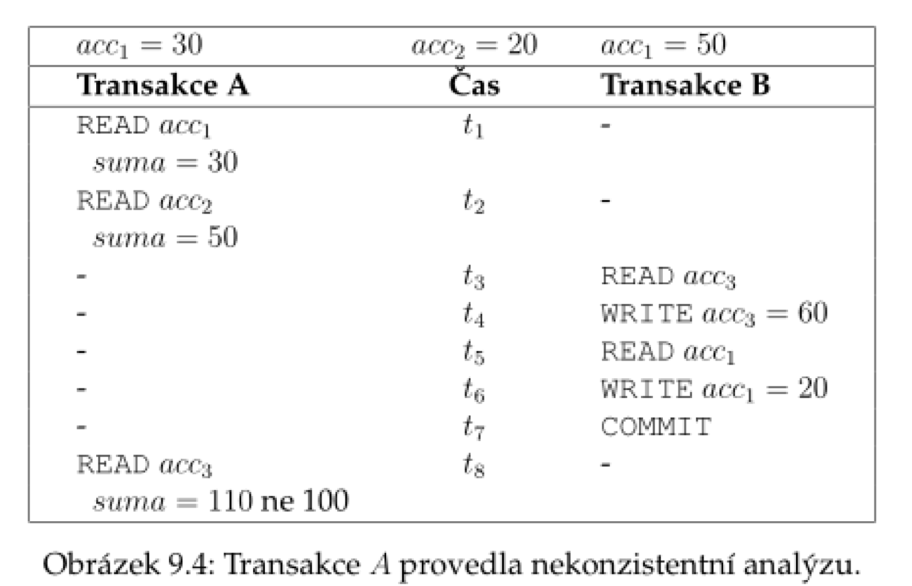
\includegraphics[width=10cm]{assets/soubeha1}}
\end{itemize}

\subsection{Konflikty čtení/zápis}
A a B chtějí \textbf{číst/zapisovat stejnou entici} (záznam). Nastávají 4 možnosti konfliktu:
\begin{itemize}
\item \textbf{RR (READ-READ)} - negativně se neovlivní, není problém.
\item \textbf{RW (READ-WRITE)} - \texttt{read\_A}, \texttt{write\_B} = A dále počítá s daty $\rightarrow$ RW zapříčiňuje \textbf{problém nekonzistentní analýzy}. \texttt{read\_A}, \texttt{write\_B}, \texttt{read\_A} $\rightarrow$ A načte odlišené hodnoty = \textbf{neopakovatelné čtení (non repeatable read)}
\item \textbf{WR (WRITE-READ)} - \texttt{write\_A}, \texttt{read\_B}, \texttt{rollback\_A}? $\rightarrow$ \textbf{Problém nepotvrzené závislosti}. Pokud B přečte data $\rightarrow$ \textbf{Špinavé čtení (dirty read)} = čtení non-commited dat.
\item \textbf{WW (WRITE-WRITE)} - \texttt{write\_A}, \texttt{write\_B}, \texttt{rollback\_A}? $\rightarrow$ \textbf{Ztráta aktualizace} (pro A) a \textbf{nepotvrzená závislost} pro B. \textbf{Špinavý zápis}\textbf{ (dirty write)} - přepisování non-commited dat.
\end{itemize}

\subsection{Techniky řízení souběhu}
\subsubsection{Správa verzí}
Předpoklad, že se paralelní \textbf{transakce ovlivňovat nebudou}. Systém \textbf{vytváří} při aktualizaci\textbf{ kopie dat }a sleduje, která z verzí má být viditelná pro ostatní transakce (podle úrovně izolace).

\subsubsection{Zamykání}
Předpokládáme, že se paralelní \textbf{transakce budou ovlivňovat}. Systém spravuje jednu kopii dat a jednotlivým transakcím přiděluje \textbf{zámky}.

\begin{itemize}
\item Chce-li transakce A provést čtení/zápis nějakého objektu v DB (nejčastěji n-tice), \textbf{požádá o zámek} na tento objekt. Žádná jiná paralelní transakce zámek získat nemůže, dokud jej A \textbf{neuvolní}.
\item \textbf{2 typy zámků:} \textbf{výlučný} zámek (exclusive lock / write lock) \textbf{X}; \textbf{sdílený} zámek (shared lock / read lock) \textbf{S}; existuje jich i více.
\item A má zámek X a B \textbf{nedostane žádný zámek} hned. A má zámek S, B \textbf{může hned dostat S}, X nikoliv.
\item \textbf{Matice kompability} - vzájemné vztahy typů zámků, sloupce a řádky: X, S, -; A (okamžitě), N (ne)
\begin{table}[H]
	\centering
	\begin{tabular}{|l|l|l|l|}
		\hline
		& X & S & - \\ \hline
		X & N & N & A \\ \hline
		S & N & A & A \\ \hline
		- & A & A & A \\ \hline
	\end{tabular}
\end{table}
\item \textbf{Operace aktualizace} - mění obsah DB - \texttt{UPDATE}, \texttt{INSERT} i \texttt{DELETE}.
\item \textbf{Uzamykací protokol} - většinou žádání zámků implicitně $\rightarrow$ při \textbf{získání} n-tice z DB žádán \textbf{zámek S}. Při aktualizaci \textbf{zámek X}; žádá-li zámek X a má už S, je mu \textbf{S změněn na X}; když nemůže být zámek přidělen okamžitě, transakce přechází do stavu \textbf{čekání} (wait state).
\item Systém musí zajistit aby v tomto stavu nesetrvala navždy - situace "\textbf{livelock}" nebo "\textbf{starvation}" $\rightarrow$ řadit požadavky do \textbf{fronty} (FIFO). Zámky uvolněny až po operaci \texttt{COMMIT} nebo \texttt{ROLLBACK}.
\item \textbf{Explicitní uzamykání} - \texttt{LOCK TABLE <names> IN [ROW SHARE|ROW EXCLUSIVE|SHARE UPDATE|SHARE|SHARE ROW EXCLUSIVE|EXCLUSIVE] MODE [NOWAIT]}
\end{itemize}

\subsection{Uváznutí}
\begin{itemize}
\item \textbf{Deadlock} - dvě nebo více transakcí jsou ve stavu \textbf{čekání} na uvolnění zámků držených jinou transakcí.
\item \textbf{Detekce uváznutí} - \textbf{časové limity} (nastavení max. času pro vykonání transakce), \textbf{detekce cyklu v grafu Wait-For} (zaznamenává, které transakce na sebe čekají $\rightarrow$ u jedné provede \texttt{ROLLBACK}).
\item \textbf{Prevence uváznutí pomocí časových razítek} - 2 verze uzamykacího protokolu. Každá transakce na začátku dostane časové razítko (unikátní). Pokud A požaduje zámek na entici, která je zamčená B pak:
\begin{itemize}
\item při \textbf{Wait-Die} - pokud je A starší než B, A přejde na čekání; je-li mladší, A je zrušena \texttt{ROLLBACK} a spuštěna znovu.
\item při \textbf{Wound-Die} - pokud A je mladší než B, A přejde na čekání; starší $\rightarrow$ B zrušena \texttt{ROLLBACK} a spuštěna znovu.
\end{itemize}
\item Při opětovném spuštění si transakce nechá své časové razítko. \textbf{Nevýhodou} je velký počet operací \texttt{ROLLBACK}. První část jména - situace kdy A je starší než B. \textbf{Nemůže nikdy dojít k uváznutí.}
\end{itemize}

\subsection{Sériový a serializovatelný plán}
\begin{itemize}
\item \textbf{Sériový plán} - n-tice uspořádaná dle \textbf{pořadí vykonávání} jednotlivých transakcí. (transakce jsou provedeny zasebou).
\item \textbf{Serializovatelný plán} - \textbf{plán vykonávání dvou transakcí} je korektní jen tehdy, pokud je serializovatelný $\rightarrow$ plán ekvivalentní s výsledkem libovolného sériového plánu.
\end{itemize}

\subsection{Úroveň izolace transakce}
Serializovatelnost garantuje izolaci transakcí ve smyslu podmínky \textbf{ACID}. Je-li plán transakcí serializovalný, neprojeví se negativní vlivy souběhu. Za izolovanost transakcí se platí \textbf{menším výkonem} souběhu $\rightarrow$ \textbf{nižší propustností}. SŘBD umožňuje nastavit úroveň izolace - ta \textbf{sníží míru izolace} transakce a \textbf{zvýší propustnost}.
\\\\
\noindent\makebox[\textwidth]{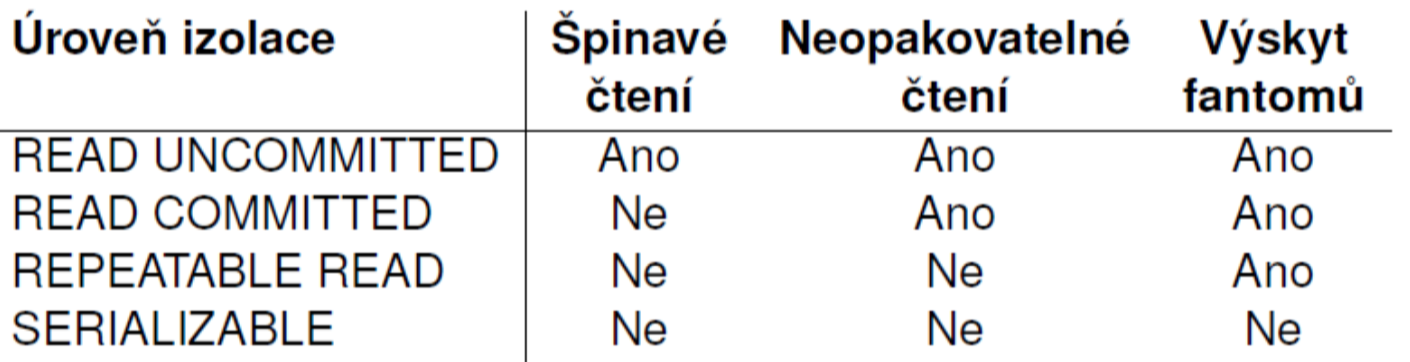
\includegraphics[width=11cm]{assets/izolace}}